\chapter{Features}
\label{chapter:features}

Now that we have an understanding about the way the n2EDM DAQ system is expected to operate we can shift the focus of our discussion to the work that was conducted over the course of this thesis. In this chapter we will explain the way they were designed and implemented, additionally highlighting their capabilities as well as the limitations the future developers and/or users might face.

\section{Support of the \texttt{FOR} loop}
\label{sec:for_loop}

\textit{Components affected}: \textbf{Sequencer} (Section \ref{sec:sequencer}).

\textit{Motivation}: While the sequencer is able to execute the pseudo-\texttt{FOR} loop as shown on the Listing \ref{listing:goto_as_for} we would still prefer to have it implemented as a standalone construction for the sake of simplicity and reducing the mental overhead of the users. Additionally the usage of \texttt{GOTO} command is generally considered \cite{Dijkstra1968} harmful, leading to the unstructured spaghetti code \cite{Cram2005}.

\begin{lstlisting}[
	caption={Implementing \texttt{FOR} with \texttt{GOTO}}, 
	label={listing:goto_as_for}, 
	language=n2EDMScript
]
SET i = 0
LABEL "FOR_START"
IF $i < 5 THEN
...
SET i = $i + 1
GOTO "FOR_START"
ELSE
ENDIF
\end{lstlisting}

\textit{Requirements}: We introduce 3 new commands that the sequencer should be able to handle:

\begin{itemize}
	\item \texttt{FOR (init; test; iterate)} or \texttt{FOR ((init; test; iterate))}. Amount of whitespace characters is arbitrary, round brackets are allowed as a part of every argument, but amount of \colorbox{selectioncolor}{\strut \texttt{(}} and \colorbox{selectioncolor}{\strut \texttt{)}} per argument needs to be balanced. Nested \texttt{FOR} blocks are allowed.
	\begin{itemize}
		\item \texttt{init}: an expression that is being executed once to init the state of the loop variable. It follows the semantic of the \texttt{SET} operator, for example \texttt{i = 0} is valid.
		\item \texttt{test}: an expression that produces a boolean value when evaluated. We run this check on every iteration, including the first one. Semantically similar to the argument of the \texttt{IF} block, so \texttt{\$i < 5} is allowed. If the output is \texttt{False}, skipping the lines until a \texttt{DONE} block is encountered. Otherwise continues execution as usual.
		\item \texttt{iterate}: an expression that is used to modify the loop variable. Gets evaluated at the end of every cycle. It borrows the structure of the \texttt{SET} command, usually using the loop variable itself in a following manner: \texttt{i = \$i + 1}
	\end{itemize}
	\item \texttt{DO}: contrary to the name it does nothing. If encountered, must have a valid \texttt{FOR} statement in a previous line of the sequence.
	\item \texttt{DONE}: marks the end of the \texttt{FOR} loop. Redirects to the beginning of the loop for the next iteration.
\end{itemize}

We should be able to replace the Listing \ref{listing:goto_as_for} with the code of the Listing \ref{listing:for_loop_example}.
\begin{lstlisting}[
	caption={Example of the \texttt{FOR} loop}, 
	label={listing:for_loop_example},
	language=n2EDMScript
]
FOR (i = 0; $i < 5; i = $i + 1)
DO
...
DONE
\end{lstlisting}

\textit{Implementation details}: 

\begin{itemize}
	\item Contrary to the implementation of the \texttt{IF/ELSE/ENDIF} blocks the \texttt{FOR} loop does not need to be complete all the times. Rather if we encounter \texttt{FOR} we evaluate the \texttt{FOR.test} condition and continue executing or skipping the next lines based on the condition's output until the matching \texttt{DONE} is found
	\item Current scope of the variables is always global, so one might prefer to use different iteration variables for nested loops to prevent confusing results
	\item Sequencer supports powerful inline editing/removal of the lines. We do not attempt to prevent cases like \texttt{GOTO} from the loop body or \texttt{REMOVELINE} of \texttt{FOR} while iterating. However the sequencer will always try to find the root of the problem and notify the user about it
	\item Default strategy for the non-parseable lines is to skip them
\end{itemize}

%\begin{lstlisting}[
%	language=JavaScript, 
%	caption={Simplified overview of the \texttt{FOR} loop implementation},
%	label={listing:for_loop_implementation}
%]
%let skipUntilDone = false
%let forDelta = 0
%
%while (canReadNextSequenceLine) {
%	++currentLineNumber
%
%	if (skipUntilDone) {
%		if (isCurrentLine('FOR')) {
%			++forDelta
%		} else if (isCurrentLine('DONE')) {
%			--forDelta
%
%			if (forDelta == 0) {
%				skipUntilDone = false
%			}
%		}
%	} else if (isCurrentLine('FOR')) {
%		setVariable(forLine.init)
%		skipUntilDone = !evaluateExpression(forLine.test)
%
%		if (skipUntilDone) {
%			forDelta = 1
%		}
%	} else if (isCurrentLine('DO')) {
%		const savedCurrentLineNumber = currentLineNumber
%		let doneDelta = 1
%
%		do {
%			--currentLineNumber
%			if (isCurrentLine('FOR')) {
%				--doneDelta
%			} else if (isCurrentLine('DONE')) {
%				++doneDelta
%			}
%		} while (!(doneDelta == 0 || currentLineNumber == 0))
%
%		if (doneDelta != 0) {
%			currentLineNumber = savedCurrentLineNumber
%		} else {
%			setVariable(forLine.iterate)
%			const canRunAgain = evaluateExpression(forLine.test)
%
%			if (!canRunAgain) {
%				currentLineNumber = savedCurrentLineNumber
%			}
%		}
%	}
%}
%\end{lstlisting}
\newpage
\section{Improved the \texttt{REQUEST} command}
\label{sec:request}

\textit{Components affected}: \textbf{Sequencer} (Section \ref{sec:sequencer}).

\textit{Motivation}: while the core functionality of this feature was provided by \cite{Germann2019} the implementation contained a few undesired restrictions:

\begin{itemize}
	\item At any given moment of time only 1 request could have been pending
	\item In order to pause the execution while request was in flight, functionality of \texttt{SLEEP} command was used. This would have lead to unexpected results when combining \texttt{SLEEP}, \texttt{PAUSE}, \texttt{RESUME} and \texttt{REQUEST} blocks.
	\item Without the Feature \ref{sec:replyto} it could have not been tested thoroughly and contained a number of bugs.
\end{itemize}

\textit{Requirements}: sequencer needs to support the \texttt{SET variable = REQUEST( question, format, timeout, default)} instruction with the semantics as described below:

\begin{itemize}
	\item \texttt{question}: required quoted string starting with \highlight{:}. Represents the node name and the  command that should return the value that we are interested in. Example: \texttt{":HV:OUTPUT:VOLTAGE?"}.
	\item \texttt{format}: optional string (\texttt{\%0} if not provided). In case the target node returns multiple comma-separated values this argument in the form of \texttt{\%n} selects the n-th element starting with 1. Special case \texttt{\%0} instructs to return the node response as a whole.
	\item \texttt{timeout}: optional int/double (\texttt{1} if not provided). Maximum amount of seconds the sequencer needs to wait for the answer.
	\item \texttt{default}: optional int/double (\texttt{0} if not provided). The value used in case the request does not return an answer within the \texttt{REQUEST.timeout}.
\end{itemize}

First step in getting the answer is sending the request itself. Let's discuss how every \texttt{REQUEST} statement should be processed before getting sent to the distributor. \texttt{REQUEST(":HV:OUTPUT:VOLTAGE?", \%2, 1, 0)} would serve us as an example:

\begin{enumerate}
	\item We select the \texttt{nodeName} from the \texttt{REQUEST.question}, in our case it would be the \texttt{:HV}, leaving \texttt{:OUTPUT:VOLTAGE?} as a \texttt{nodeCommand}
	\item{
		We create a quoted \texttt{argumentsString} which looks like 
		\begin{verbatim}
			"sequencerNodeName:RESULT requestId, REQUEST.format"
		\end{verbatim}
		\begin{itemize}
			\item \texttt{sequencerNodeName} is the name with which the sequencer was registered with the distributor, let's assume it is \texttt{SEQUENCER}.
			\item \texttt{requestId} is a unique positive integer used to distinguish the received answers, we would select 17.
		\end{itemize}
		In our case \texttt{argumentsString} would be \texttt{"SEQUENCER:RESULT 17, \%2"}
	}
	\item{
		We create a final \texttt{requestCommand} of the shape
		\begin{verbatim}
			nodeName:REPLYTO(argumentsString)nodeCommand
		\end{verbatim}
		or for the example that we have started with
		\begin{verbatim}
			HV:REPLYTO("SEQUENCER:RESULT 17, %2"):OUTPUT:VOLTAGE?
		\end{verbatim}
	}
	\item The \texttt{requestCommand} is sent to the distributor.
\end{enumerate}

Second step is receiving the answer. To do that, sequencer supports the \texttt{RESULT} command. Following the example we expect to receive a string \texttt{RESULT 17, remoteValue} and execute \texttt{SET variable = remoteValue}. One could notice that the node answer looks like if the \texttt{argumentsString} from above would have been used as a template.

Sequencer supports 2 sources of commands, called external and internal. External commands are the one that arrive from the distributor. Internal commands come from a sequence of commands that the sequencer stores in memory. A command can be loaded into this sequence from the external commands, for example with \texttt{ADDLINE "..."}. For this feature we are only interested in a subset of commands from both sides:

\begin{itemize}
	\item \textbf{External}:
	\begin{itemize}
		\item \texttt{PAUSE}. Pauses the execution of all internal commands until the \texttt{RESUME} is received.
		\item \texttt{RESUME}. Resumes the execution of all internal commands if paused by \texttt{PAUSE}.
		\item \texttt{RESTART}. New command, removes information about all requests, rewinds the internal sequence to the first line, cancels any blocks introduced by \texttt{PAUSE} or \texttt{SLEEP}. \textbf{Preserves} the state of all variables.
		\item \texttt{SET variable = REQUEST(...)}. Pauses the execution of the internal commands until either an answer is returned or the timeout of the corresponding request was reached, whatever event happens earlier. Sets the variable to the received or default value.
	\end{itemize}
	\item \textbf{Internal}:
	\begin{itemize}
		\item \texttt{SLEEP ...s}. Pauses the execution of the internal sequence for a given amount of seconds. Is \textbf{not} equal to pausing the sequencer with \texttt{PAUSE}.
		\item \texttt{SET variable = REQUEST(...)}. Same logic as if it would have been executed directly from the external source.
	\end{itemize}
\end{itemize}

\newpage

\textit{Implementation details}:

\begin{itemize}
	\item{
		The execution of the internal sequence can be paused independently by multiple events:
		\begin{enumerate}
			\item \texttt{PAUSE} and reaching the end of the sequence set the internal \texttt{isPaused} flag to \texttt{True}.
			\item \texttt{SLEEP} sets the \texttt{isSleeping} flag to \texttt{True} and saves the time at which it should be set back to \texttt{False}.
			\item At least 1 pending request is in flight.
		\end{enumerate}
		The execution continues only in case of none of these blocking conditions being present.
	}
	\item{
		A somewhat unexpected consequence of sharing the \texttt{SET} logic is that the \texttt{REQUEST} can be also used as part of the Feature \ref{sec:for_loop}. Both \texttt{FOR.init} and \texttt{FOR.iterate} can be \texttt{REQUEST}ed, making the following line valid:
\begin{lstlisting}[language=n2EDMScript, numbers=none]
FOR (i = REQUEST(...); $i < 5; i = REQUEST(...))
\end{lstlisting}
	}
\end{itemize}

%In the Listing \ref{listing:request} we present a skeleton that handles the sending/receival of the requests as well as the management of the execution state.

%\begin{lstlisting}[
%	language=JavaScript,
%	caption={Simplified overview of the \texttt{REQUEST} command implementation},
%	label={listing:request}
%]
%interface RequestMetadata {
%	id: number
%	isActive: boolean
%	variableName: string
%	defaultValue: string
%	start: Date
%	deadline: Date
%}
%
%const requests = new Map<number, RequestMetadata>()
%let currentRequestId = 1
%
%function getPendingRequests() {
%	const result: RequestMetadata[] = []
%
%	for (const request of requests.values()) {
%		if (request.isActive) {
%			result.push(request)
%		}
%	}
%
%	return result
%}
%
%function areRequestsPending() {
%	const pendingRequests = getPendingRequests()
%
%	if (pendingRequests.length > 0) {
%		return true
%	} else {
%		return false
%	}
%}
%
%function cleanRequests() {
%	requests.clear()
%}
%
%function sendRequestToDistributor(
%	question: string,
%	format: string,
%	timeout: string,
%	defaultValue: string,
%	variableName: string
%) {
%	++currentRequestId
%
%	const command = createReplyToCommand(
%		question,
%		currentRequestId,
%		format,
%		defaultValue
%	)
%
%	const deadline = addSeconds(new Date(), timeout)
%	requests.set(currentRequestId, {
%		id: currentRequestId,
%		isActive: true,
%		variableName,
%		defaultValue,
%		start: new Date(),
%		deadline
%	})
%
%	sendCommand(command)
%}
%
%function handleDistributorResponse(
%	responseId: number, 
%	responseValue: string
%) {
%	const request = requests.get(responseId)
%
%	if (new Date() > request.deadline) {
%		requests.delete(responseId)
%		return
%	}
%
%	setVariable(request.variableName, responseValue)
%	requests.delete(responseId)
%}
%
%function checkRequestTimeout() {
%	const pendingRequests = getPendingRequests()
%
%	for (const request of pendingRequests) {
%		if (new Date() > request.deadline) {
%			setVariable(request.variableName, request.defaultValue)
%			request.isActive = false
%		}
%	}
%}
%
%function setVariable(expression: string) {
%	if (isCommand(expression, 'REQUEST')) {
%		sendRequestToDistributor(
%			question,
%			format,
%			timeout,
%			defaultValue,
%			variableName
%		)
%	}
%}
%
%let isPaused = true
%let isSleeping = false
%let endOfSleep = new Date()
%
%function analyse(command: string) {
%	if (isCommand(command, 'PAUSE')) {
%		isPaused = true
%	} else if (isCommand(command, 'RESUME')) {
%		isPaused = false
%	} else if (isCommand(command, 'RESTART')) {
%		isPaused = false
%		isSleeping = false
%		currentLineNumber = 0
%		cleanRequests()
%	} else if (isCommand(command, 'SET')) {
%		setVariable(command)
%	} else if (isCommand(command, 'RESULT')) {
%		handleDistributorResponse(responseId, responseValue)
%	}
%}
%
%function resume() {
%	const blockedByRequests = areRequestsPending()
%
%	if (!isPaused && !isSleeping && !blockedByRequests) {
%		if (!canReadNextSequenceLine) {
%			isPaused = true
%		} else {
%			++currentLineNumber
%
%			if (isCurrentLine('SLEEP')) {
%				endOfSleep = addSeconds(new Date(), seconds)
%			} else if (isCurrentLine('SET')) {
%				setVariable(expression)
%			}
%		}
%	}
%
%	if (isSleeping) {
%		if (new Date() > endOfSleep) {
%			isSleeping = false
%		}
%	}
%
%	if (blockedByRequests) {
%		checkRequestTimeout()
%	}
%}
%
%while (!shouldExit) {
%	const command = readOneExternalCommand()
%
%	if (command.length > 0) {
%		analyse(command)
%	} else {
%		resume()
%	}
%}
%\end{lstlisting}

\section{Implemented the \texttt{REPLYTO} command}
\label{sec:replyto}

\textit{Components affected}: \textbf{COM Handler} (Section \ref{sec:com_handler})

\textit{Motivation}: in order to create a truly interconnected DAQ system it is not enough to be able to send SCPI commands to our nodes. We also need to be able to use their responses for a feedback loop of any kind. By implementing this feature on the COM handler level it  would be possible to return a response of any node.

\textit{Requirements}: following the contract of the \texttt{REQUEST} Feature \ref{sec:request} the COM handler needs to support a \texttt{:REPLYTO} command. We would like to achieve a behaviour as described below:

\begin{itemize}
	\item Only one \texttt{:REPLYTO} command can be processed at a time. When it is executed the COM handler should continue accepting commands from the distributor. These commands would be buffered in memory until the pending \texttt{:REPLYTO} command completes.
	\item{
		Given the example from the Feature \ref{sec:request}
		\begin{verbatim}
			HV:REPLYTO("SEQUENCER:RESULT 17, %2"):OUTPUT:VOLTAGE?
		\end{verbatim}
		we will send \texttt{OUTPUT:VOLTAGE?} to the node and pause the further execution of the SCPI commands.
	}
	\item{
		Upon executing the \texttt{:REPLYTO} command the COM handler sets a time window based on the integer \texttt{scpiResponseTimeoutMs} value from the config file \texttt{conf\_n2comhandler.cfg}. We have 3 cases to handle:
		\begin{itemize}
			\item If nothing came over the SCPI connection with the node during the waiting interval then it means that \texttt{:REPLYTO} has timed out. We resume the execution of the SCPI commands from the distributor from the next command, if any.
			\item If a complete message that starts with \highlight{:} was received then we assume that the node is trying to communicate with other components of the system. Such message is forwarded to the distributor directly as is and does not influence the \texttt{:REPLYTO} feature flow.
			\item Otherwise if a complete message was received while we are still within the time window of waiting for response then we consider it to be an answer to the \texttt{:REPLYTO} being in flight.
			\item If a node answer that does not start with \highlight{:} was received outside of the \texttt{:REPLYTO} timeout the COM handler would skip it and print a warning.
		\end{itemize}
		\item{
			If a complete SCPI response was received in time then our next task is to parse it. A node might decide to return multiple comma-separated values. We split the message into chunks by using the rules below:
			\begin{itemize}
				\item Message is scanned from left to right
				\item Splittable parts are separated by commas \highlight{,}
				\item Escaped commas \highlight{\textbackslash ,} are not separators
				\item Commas that appear inside of a string are not separators
				\item String starts with a quotation mark \highlight{"}
				\item String might end with a quotation mark \highlight{"}. If there is no closing quotation mark, we consider the string to end at the end of the message. So in \texttt{"1,2,3} none of the commas would be a separator
				\item Escaped quotation marks \highlight{\textbackslash "} are not considered quotation marks
			\end{itemize}
		}
		\item{
			After splitting the message we need to extract the correct \texttt{answerValue} by using the format argument, in our example that would be \texttt{\%2}
			\begin{itemize}
				\item \texttt{\%0} means that no splitting is required and \texttt{answerValue} is set to the received message as a whole
				\item \texttt{\%n} means that \texttt{answerValue} is set to the \texttt{n}-th part of the split message with count starting with 1. If the message contained no separators then \texttt{\%0} and \texttt{\%1} produce the equal output. If the split message contains less than \texttt{n} parts we set \texttt{answerValue} to an empty unquoted string.
			\end{itemize}
		}
		\item After extracting the \texttt{answerValue} we are ready to send back the answer. Let's assume that \texttt{answerValue = 289}. Following our example, the COM handler will need to send \texttt{:SEQUENCER:RESULT 17, 289} over FIFO to the distributor.
	}
\end{itemize}

\textit{Implementation details}:

\begin{itemize}
	\item{
		In the \textit{requirements} above one can often see a combination of words \textbf{complete message}. Neither TCP/IP nor FIFO files guarantee that the message sent as one would be received as one. All SCPI messages, such as
		\begin{itemize}
			\item Commands from the distributor
			\item Answers to the distributor
			\item Command to the node
			\item Answers from the node
		\end{itemize}
		must use a newline \highlight{\textbackslash n} symbol to indicate the ending of the command. Internally we have 2 string buffers: for the commands from the distributor and the answers from the node. Every received message is placed into a corresponding buffer. On every tick we attempt to select one \textbf{complete} message by splitting once on the newline symbol \highlight{\textbackslash n} starting from the beginning of the buffer. In case of success this \textbf{complete} message is placed in a corresponding sequence and treated as a SCPI command/answer. The SCPI answers buffer is not cleaned on the \texttt{:REQUEST} timeout.
	}
	\item We consider a SCPI response to be an answer to \texttt{:REPLYTO} if it was received during the timeout window. Even though the default value of \texttt{scpiResponseTimeoutMs} being 5000 should be enough for the node to return the answer in time, we cannot guarantee it. Thus a very late answer that comes during the execution of the \textbf{next} \texttt{:REPLYTO} command would be sent as an answer to the distributor.
	\item{
		Combining both points we might get a very confusing situation:
		\begin{enumerate}
			\item COM handler executes first \texttt{:REPLYTO}
			\item Node sends back \texttt{verylonganswer\textbackslash n}
			\item The answer does not fit in a single package and the COM handler received only \texttt{very} and adds it to the answer buffer.
			\item Due to the network error the connection between the node and the COM handler is broken. First \texttt{:REPLYTO} times out.
			\item Network connection is reestablished
			\item COM handler executes second \texttt{:REPLYTO}
			\item Node sends back \texttt{shortanswer\textbackslash n}
			\item Depending on the node logic, 2 situations would be possible:
			\begin{itemize}
				\item Node tries to send the remaining \texttt{longanswer\textbackslash n} first. COM handler would have an answer buffer \texttt{verylonganswer\textbackslash n} and send it as a result of the second \texttt{:REPLYTO}. The received message \texttt{shortanswer\textbackslash n} would be appended to the buffer and depending on timing either ignored or sent as a reply to the third \texttt{:REPLYTO}
				\item Node skips the \texttt{longanswer\textbackslash n} and decides to respond only with \texttt{shortanswer\textbackslash n}. COM handler would have an answer buffer \texttt{veryshortanswer\textbackslash n} and return it as a result of the second \texttt{:REPLYTO}.
			\end{itemize}
		\end{enumerate}
		One can see that with a lot of requests and slow nodes that might become an issue, thus the COM handler would print a warning if its queue of the pending SCPI commands has more than one item.
	}
\end{itemize}
\section{Implemented the sequencer's TCP/IP interface}
\label{sec:tcp_ip_sequencer}

\textit{Components affected}: \textbf{Sequencer} (Section \ref{sec:sequencer})

\textit{Motivation}: connecting the sequencer directly to the distributor via the POSIX pipes would require us to implement the logic that handles it twice: in both the sequencer and the COM handler. In order to reduce complexity we would prefer the sequencer to behave as a regular node that uses a COM handler proxy for the communication with other parts of the DAQ system.

\textit{Requirements}: sequencer needs to act as a TCP/IP server by listening on 2 ports: one for the SCPI commands and one for the data connection. The only connection that would be used is the SCPI connection. Values for the corresponding port numbers should be provided via a \texttt{libconfig}-compliant configuration file.

\textit{Implementation details}: a configuration file \texttt{conf\_n2comhandler.cfg} of the COM handler would serve us as an example. Following it we introduce \texttt{conf\_sequencer.cfg} that needs to be present in the same folder as the \texttt{sequencer} executable. It must contain the following fields:

\begin{itemize}
	\item \texttt{name} string --- a short human-readable description of the sequencer.
	\item \texttt{moduleName} string --- is required to provide a \texttt{sequencerNodeName} in the Feature \ref{sec:request}. Must be equal to the \texttt{moduleName} of the corresponding COM handler config.
	\item \texttt{ipAddr} string --- an interface that the sequencer needs to be listening on, for example \texttt{127.0.0.1}. Might be marked obsolete by modifying the sequencer code to listen on all network interfaces. In this case it would be ignored and thus one could completely reuse the \texttt{conf\_n2comhandler.cfg}.
	\item \texttt{cmdPort} integer --- a port number for the TCP server to listen for the SCPI commands.
	\item \texttt{dataPort} integer --- a port number for the TCP server to accept the data connection. Following the example of the COM handler a default value of 50250 was used. However as it was later found during the implementation of the Feature \ref{sec:com_handler_network_errors} a value outside of the ephemeral port range would be preferred.
\end{itemize}

We provide an example of the configuration file that uses the default values below on the Listing \ref{listing:sequencer_config}:

\begin{lstlisting}[
	caption={Example of the \texttt{conf\_sequencer.cfg}},
	language=n2EDMScript,
	label={listing:sequencer_config}
]
name = "sequencer - a n2EDM scheduler for SCPI commands";
moduleName = "SEQUENCER";
ipAddr = "127.0.0.1";
cmdPort = 5025;
dataPort = 50250;
\end{lstlisting}

It is important to notice that in the current setup the sequencer would wait for the TCP connections only on the start of the execution. Any network error or disconnection of the COM handler would cause the sequencer to print a warning and exit. Whether the sequencer needs to handle these cases differently is up for discussion.
\section{Improved the COM handler's networking}
\label{sec:com_handler_network_errors}

\textit{Components affected}: \textbf{COM handler} (Section \ref{sec:com_handler}).

\textit{Motivation}: we live in a world where the network errors are part of the reality. It is unacceptable for the COM handler being one of the most important communication bridges in the DAQ system to shut down in case of the connected node becoming unreachable over the network.

\textit{Requirements}: instead of a single attempt to connect to the node when being started the COM handler needs to graciously manage the corresponding network connections:

\begin{itemize}
	\item SCPI and data connections are managed in a same fashion but independently, errors in one of them should not affect the other.
	\item We try connecting to the node as many times as needed to establish a network link.
	\item If the COM handler encounters an error in the SCPI or data connection it should properly close it and start reconnecting.
	\item If the error was raised in the SCPI connection while sending a command to the node, this command should not be lost but rather resent as a first message when a new SCPI connection is established.
\end{itemize}

\textit{Implementation details}:

\begin{itemize}
	\item{
		\texttt{:REPLYTO} commands are sent to the node when the SCPI connection becomes available. The deadline for the node response is calculated at the moment of sending the command. When set, the time window does not account for the disconnects:
		\begin{enumerate}
			\item Waiting time is 5 seconds.
			\item At time $T$ the COM handler sends the SCPI command to the node.
			\item At time $T + 1$ seconds the SCPI link goes down.
			\item At time $T + 5$ seconds the COM handler considers the request to be expired.
			\item At time $T + 6$ seconds the SCPI connection is reestablished.
			\item At time $T + 7$ seconds the node returns the answer but it is not considered valid, even though the waiting time with the \textbf{open} SCPI connection was only 2 seconds.
		\end{enumerate}
	}
	\item Persistent attempts of the COM handler to open a data connection to the \texttt{127.0.0.1} without the node being reachable might lead to an unexpected outcome --- the connection would be established with the COM handler itself! As briefly mentioned in the Feature \ref{sec:tcp_ip_sequencer} it has to do with the fact that the default data port number used to be in the ephemeral port range \cite{RichardStevens1998}. Although such behaviour is consistent with the RFC \cite{Postel1981} it is not desired while operating the DAQ system. One is advised to use both the SCPI and the data ports outside of the ephemeral range in order to prevent confusions.
\end{itemize}
\section{Improved the \texttt{SHOWVARIABLES?} command}
\label{sec:showvariables}

\textit{Components affected}: \textbf{Sequencer} (Section \ref{sec:sequencer}).

\textit{Motivation}: with the Features \ref{sec:replyto} and \ref{sec:tcp_ip_sequencer} implemented it becomes possible to use the sequencer's output by other nodes. One of the things that might be of interest is the snapshot of the variables of the sequencer.

\textit{Requirements}: the sequencer needs to handle the \texttt{SHOWVARIABLES?} command by sending a single string over the SCPI connection. This message is created with the following rules in mind:

\begin{itemize}
	\item Any variable forms a string \texttt{variableName=variableValue}.
	\item An additional variable \texttt{LINE\_EXECUTED\_NEXT} is included. Its value is defined as the number of the line in the \textbf{internal} sequence (more details in the Feature \ref{sec:request}) that would be executed afterwards. The count starts with 0.
	\item All individual chunks are joined by using \highlight{|} as a separator.
\end{itemize}

\textit{Implementation details}: assuming that the sequencer is registered with the distributor under the name \texttt{SEQUENCER} and the distributor's main FIFO file path is \texttt{/n2edm/\_n2sim\_input} the following set of the shell commands:

\begin{lstlisting}[language=bash]
	echo "SEQUENCER:ADDLINE SET x = 17" >> /n2edm/_n2sim_input
	echo "SEQUENCER:ADDLINE SET y = 289" >> /n2edm/_n2sim_input
	echo "SEQUENCER:RESUME" >> /n2edm/_n2sim_input
	sleep 5
	echo "SEQUENCER:SHOWVARIABLES?" >> /n2edm/_n2sim_input
\end{lstlisting}

would cause the sequencer to send back this string over SCPI:

\begin{verbatim}
	LINE_EXECUTED_NEXT=2|x=17.000000|y=289.000000\n
\end{verbatim}

One can see that the sequencer has correctly executed 2 \texttt{SET} lines and now the \texttt{LINE\_EXECUTED\_NEXT} is pointing to the virtual third line which represents the end of the sequence.
\section{Improved the \texttt{SHOWLINES?} command}
\label{sec:showlines}

\textit{Components affected}: \textbf{Sequencer} (Section \ref{sec:sequencer}).

\textit{Motivation}: similar to the Feature \ref{sec:showvariables} we would like to return the information about the lines of the internal sequence over the SCPI connection.

\textit{Requirements}: we process the lines for \texttt{SHOWLINES?} command almost like we process the variables for the \texttt{SHOWVARIABLES?} command. There are, however, a few differences to keep in mind:

\begin{itemize}
	\item Syntax of individual chunks is changed to \texttt{lineNumber:lineValue} with \texttt{lineNumber} starting from 0.
	\item \texttt{LINE\_EXECUTED\_NEXT} needs to be added as a virtual \texttt{lineNumber}.
	\item Line chunks are joined by using \highlight{|} as a separator.
	\item When joining the lines all virtual lines need to be in the beginning. Real lines following the virtual lines block need to be presented in the same order as they are kept in the sequencer's memory.
	\item{
		Contrary to the variable names and values, the \texttt{lineValue} might contain \highlight{|} and thus it could be escaped. We use a logic that somewhat resembles the one presented in the Feature \ref{sec:replyto}:
		\begin{itemize}
			\item The line needs escaping if it contains at least one qualified \highlight{|}.
			\item The line content is scanned from left to right	.
			\item Escaped separators \highlight{\textbackslash |} do not qualify.
			\item Symbol \highlight{|} that appears inside of a string does not qualify.
			\item String starts with a quotation mark \highlight{"}.
			\item String might end with a quotation mark \highlight{"}. If there is no closing quotation mark, we consider the string to end at the end of the line. So in \texttt{"text|moretext|} none of the \highlight{|} would qualify.
			\item Escaped quotation marks \highlight{\textbackslash "} are not considered quotation marks.
		\end{itemize}
	}
	\item{
		If the line's content needs escaping, we would form the \texttt{lineValue} by following these rules:
		\begin{enumerate}
			\item All double quotes \highlight{"} are transformed into \highlight{\textbackslash "}.
			\item Escaped content is placed between two quotation marks \highlight{"}.
		\end{enumerate}
	}
\end{itemize}

\textit{Implementation details}: assuming the same configuration as in the Feature \ref{sec:showvariables} we can execute

\begin{lstlisting}[language=bash]
	echo "SEQUENCER:ADDLINE SET x = 17" >> /n2edm/_n2sim_input
	echo "SEQUENCER:ADDLINE SET y = 289" >> /n2edm/_n2sim_input
	echo "SEQUENCER:RESUME" >> /n2edm/_n2sim_input
	sleep 5
	echo "SEQUENCER:SHOWLINES?" >> /n2edm/_n2sim_input
\end{lstlisting}

to order the sequencer to reply with:

\begin{verbatim}
	LINE_EXECUTED_NEXT:2|0:SET x = 17|1:SET y = 289\n
\end{verbatim}

As expected, the value of the \texttt{LINE\_EXECUTED\_NEXT} is consistent with the one that can be received as an answer to the \texttt{SHOWVARIABLES?} command.
\newpage
\section{Implemented the remote magnetometers' proxy}
\label{sec:rm-proxy}

\url{https://gitlab.com/n2edm/remote-magnetometers-proxy}

\begin{figure}[h]
	\includegraphics[width=\textwidth]{img/remote_magnetometers_proxy_schema}
	\caption{Position of the remote magnetometers' proxy in the n2EDM DAQ system.}
	\label{fig:rm-proxy_position}
\end{figure}

\textit{Magnetometers' code}: \url{https://gitlab.com/n2edm/remote-magnetometers}

\textit{Overview}: the remote magnetometers' proxy, or the \textbf{RM-proxy} for brevity, aims to be a missing link between the master node orchestrating a pool of Raspberry Pis with sensor panels and the standard TCP/IP interface of the COM handler. The remote-magnetometers project was already connected to the old LabVIEW \textbf{nEDM} DAQ system, however with this adapter it becomes possible to integrate it into the new \textbf{n2EDM} DAQ system.

\textit{General principles}: in order to make the RM-proxy robust and ideally allow it to run without downtime over the whole course of the n2EDM experiment the values below were adopted:

\begin{itemize}
	\item \textbf{Handle errors} --- errors happen and the RM-proxy is not an exception. We attempt to graciously process them, for example a problem with the TCP or ZeroMQ link should lead to closing and recreating the corresponding connection. Additionally every handleable issue should generate and save a report message that can be retrieved for an error analysis. Potentially later the n2EDM DAQ system would have a dedicated exception node to process those.
	\item \textbf{Zero data loss} --- in an experiment as complex as the n2EDM experiment every single bit of data might improve the precision of the result. Thus it is essential that the data processing and communication are decoupled from each other. Network issues should never lead to the data loss, rather the data chunk should be saved in the memory and a new attempt to send it should be made when a healthy connection is established again.
	\item \textbf{Trust the newer} --- the connected COM handler might get stuck or experience other issues that would not lead to it closing the network connection. The RM-proxy considers every new client to be the healthiest one by properly closing older connections and only allowing a single COM handler to be connected at any given moment of time.
\end{itemize}

\subsection{SCPI interface}
\label{subsec:rm-proxy_scpi}

\textit{Motivation}: even though at the current stage the RM-proxy is a passive client of the magnetometers' master node we would still like to have a working SCPI connection for the potential future tasks, for example to be able to remotely update the firmware on the magnetometers.

\textit{Requirements}: by following the SCPI specification \cite{SCPIConsortium1999} we aim to support a single \texttt{SYStem:ERRor[:NEXT]?} command which comes in multiple flavours:

\begin{itemize}
	\item \texttt{SYSTem:ERRor?}
	\item \texttt{SYST:ERR?}
	\item \texttt{SYSTem:ERRor:NEXT?}
	\item \texttt{SYST:ERR:NEXT?}
\end{itemize}

Any of the commands above replies with a message of the following format:
\begin{verbatim}
code, "event_description;[event_info;]date"
\end{verbatim}
where
\begin{itemize}
	\item \texttt{code}, required integer --- an error code from \cite{SCPIConsortium1999} that aims to provide the closest definition of the type of the issue occurred, e.g.\ \texttt{-360}.
	\item \texttt{event\_description}, required string --- a human-readable description of the \texttt{code} as specified in \cite{SCPIConsortium1999}, e.g.\ \texttt{Communication error}.
	\item \texttt{event\_info}, optional string --- custom metadata that we might add to precisely describe the reason of raising the error, e.g.\ \texttt{Error in the SCPI connection!}.
	\item \texttt{date}, required string --- a \texttt{yyyy/mm/dd HH:MM:SS.sss} timestamp \cite{SCPIConsortium1999} of the moment the error message was created.
\end{itemize}

Internally errors are stored in a FIFO queue with a size limit of $10^5$ units. If the queue is full and we attempt to write a new message then the last message in the queue is replaced with a \texttt{-350, "Queue overflow;date"} with the \texttt{date} following the rules above.

When processing the  \texttt{SYStem:ERRor[:NEXT]?} command we attempt to pick a first message in the error queue to be used as a SCPI answer. If the queue is empty we return \texttt{0, "No error;date"} where the \texttt{date} is constructed at the moment of processing the command as it was defined before.

\textit{Implementation details}: if the network connection is broken when we try sending back \texttt{0, "No error;date"} then this message would be placed in the FIFO queue together with the corresponding network error to be resent later.

\subsection{Data interface}
\label{subsec:rm-proxy_data}

\textit{Motivation}: in order to store the data collected by the remote magnetometers we need to pack it into the appropriate \cite{Bison2018} binary format and send to the COM handler over the TCP data connection.

\textit{Requirements}: we expect the messages received from the master node over the ZeroMQ connection to look like \texttt{node\_message; node\_message; \ldots} and to contain as many \texttt{node\_message}s as there are the remote magnetometers connected. Every \texttt{node\_message} can either be a \texttt{nan} string if the root node was not able to acquire the individual node measurements in time or a space-separated string \texttt{value\_1 value\_2 \ldots} otherwise, with every \texttt{value\_*} being a float. We provide a more detailed information about them in the Table \ref{tbl:node_message}:

\begin{table}[h]
\centering
\begin{tabular}{|r|l|l|}
	\hline
	Position & Description & Units \\
	\hline \hline
	1 & Timestamp of the node & seconds \\
	\hline
	2 & Magnetic field $x$ & $\mu$T \\
	\hline
	3 & Magnetic field $y$ & $\mu$T \\
	\hline
	4 & Magnetic field $z$ & $\mu$T \\
	\hline
	5 & Temperature & $^\circ$C \\
	\hline
	6 & Pressure & mbar \\
	\hline
	7 & Humidity & \% \\
	\hline
	8 & Rotational speed $x$ & radians/second \\
	\hline
	9 & Rotational speed $y$ & radians/second \\
	\hline
	10 & Rotational speed $z$ & radians/second \\
	\hline
	11 & Acceleration $x$ & Gs \\
	\hline
	12 & Acceleration $y$ & Gs \\
	\hline
	13 & Acceleration $z$ & Gs \\
	\hline
\end{tabular}
\caption{Structure of the \texttt{node\_message}.}
\label{tbl:node_message}
\end{table}

\textit{Implementation details}: we need to process the received message and pack it into the format that the COM handler would understand. Let us take a look at the n2EDM DAQ specification \cite{Bison2018}. We see that every separate field in the joint binary data message needs to be presentable as a 64 bit value with the first one always being a timestamp in nanoseconds since 1970, usually in \texttt{uint64}. Luckily we can \cite{WorkingGroupforFloating-PointArithmetic1985} represent the \texttt{NaN} value as a \texttt{double} thus we will attempt to construct a structure of the following shape:
\[
\underbrace{\texttt{timestamp}}_{\texttt{uint64}}
\ 
\underbrace{\vphantom{\texttt{timestamp}} \texttt{value\_*}}_{\texttt{double} \times 13 \times \text{number of magnetometers}}
\]

We define the \texttt{timestamp} as a minimal time among all the \texttt{node\_message}s being present in a single ZeroMQ message. But one inevitably needs to handle the case of every \texttt{node\_message} in a package being \texttt{nan}, we would refer to such packages as \textbf{empty}. The specification for dealing with them is presented below:

\begin{enumerate}
	\item{
		On the RM-proxy start we wait for the first non-empty package. All empty messages received before that moment would be thrown away during the processing stage.
		\begin{enumerate}
			\item We use the \texttt{timestamp}s of individual \texttt{node\_message}s to calculate and cache the \texttt{timestamp} of the binary message that would be later sent to the COM handler.
			\item Repeat the previous step until an empty message is received.
		\end{enumerate}
	}
	\item{
		On this step the RM-proxy needs to handle an empty message.
		\begin{enumerate}
			\item Following the Section \ref{sec:timing_infrastructure} we can calculate a new \texttt{timestamp} by using the refresh rate of the master node and a cached value of the preceding package's \texttt{timestamp}.
			\item We cache the new \texttt{timestamp}.
			\item{
				\textit{Was the previous message of the master node empty?}
				\begin{itemize}
					\item \textbf{Yes} --- this empty message is skipped to save the disk space.
					\item \textbf{No} --- we will send the first empty (only a timestamp is included) binary package to the COM handler. The warning is added to the error queue of the Feature \ref{subsec:rm-proxy_scpi}.
				\end{itemize}
			}
			\item Repeat until a first non-empty message is received.
		\end{enumerate}
	}
	\item On a first non-empty message we go to the first step.
\end{enumerate}

\subsection{Generation of the configs}
\label{subsec:rm-proxy_configs}

\textit{Motivation}: we have 3 projects that share the configuration data: RM-proxy, COM handler and the master node. Apart from them, a configuration for the COM handler requires the specification for every binary field of the data package from the Feature \ref{subsec:rm-proxy_data}. One can see that the total number of fields to fill $1 + 13 \times N$, where $N$ is the number of magnetometers, quickly becomes unmaintainable by hand and error-prone.

\textit{Requirements}: to solve these issues we introduce a single source of truth: a root config and a script that handles other configs as the build artefacts. The root config is written in a \texttt{libconfig}-compatible format. 

\textit{Implementation details}: Assuming that one is in the root of the RM-proxy's repository we will take a look at the \texttt{src/root\_config.cfg} on the Listing \ref{listing:rm-proxy_root} and explain every field.

\begin{lstlisting}[
	language=JavaScript,
	caption={Root config of the RM-proxy project.},
	label={listing:rm-proxy_root}
]
moduleName = "MAGNETOMETERS";
proxyIpAddress = "127.0.0.1";
proxyScpiPort = 5025;
proxyDataPort = 5026;

masterNodeIp = "192.168.0.254";
masterNodeBroadcastPort = 40003;

nodes = (
    {
        number: 1,
        location: "On the table (left)",
        disabled: true
    },
    {
        number: 2,
        location: "On the table (center)",
        disabled: false
    },
    {
        number: 3,
        location: "On the table (right)",
        disabled: false
    },
    {
        number: 4,
        location: "Under the table",
        disabled: false
    }
);
\end{lstlisting}

\begin{itemize}
	\item \texttt{moduleName}, required string --- a name under which the COM handler would register itself with a distributor.
	\item \texttt{proxyIpAddress}, required string --- is the IP address of the RM-proxy by using which the COM handler can connect to it.
	\item \texttt{proxyScpiPort} and \texttt{proxyDataPort}, required integers --- define on what ports should the RM-proxy listen and the COM handler should try connecting to.
	\item \texttt{masterNodeIp}, required string and \texttt{masterNodeBroadcastPort} required integer --- define the IP and broadcast port of the ZeroMQ endpoint of the master node, to which the RM-proxy connects.
	\item{
		\texttt{nodes}, array --- describes the properties of the worker nodes. Every object might contain the following fields:
		\begin{itemize}
			\item \texttt{number}, required integer --- is used to generate the IP address in the format \texttt{192.168.0.number} and the node name \texttt{mag\_number}. The node name is included in the header file generated by the COM handler as a column name, e.g.\ \texttt{humidity @ mag\_2}.
			\item \texttt{location}, required string --- refers to the physical location of the magnetometer. This is included in the header file generated by the COM handler as a column description, e.g.\ \texttt{[\%] @ On the table (center)}.
			\item \texttt{disabled}, optional boolean (default: \texttt{false}) --- allows to mark a single node as excluded from the data collection. Setting this value to \texttt{true} would not include the information about this node into any of the generated configs.
			\item \texttt{controlPort}, optional integer (default: \texttt{40001}) --- the control port of the magnetometer node.
			\item \texttt{queryPort}, optional integer (default: \texttt{40002}) --- the query port of the magnetometer node.
			\item \texttt{broadcastPort}, optional integer (default: \texttt{40003}) --- the broadcast port of the magnetometer node.
			\item \texttt{logPort}, optional integer (default: \texttt{40004}) --- the log port of the magnetometer node.
		\end{itemize}
	}
\end{itemize}

In order to generate the configs one needs to run a following command from the repository's root:
\begin{verbatim}
python3 src/generate_configs.py
\end{verbatim}
This would read \texttt{src/root\_config.cfg} and create or overwrite 3 configs:

\begin{itemize}
	\item \texttt{generated/conf\_magnetometers\_proxy.cfg} is for the RM-proxy.
	\item \texttt{generated/conf\_n2comhandler.cfg} is for the COM handler.
	\item \texttt{generated/nodes.txt} is for the master node.
\end{itemize}




\section{Improved the SFC system}
\label{sec:sfc}

\url{gitolite@nedm.psi.ch:babySFC}

\textit{Overview}: Surrounding Field Compensation \cite{Franke2013, Rawlik2018a} system, or the \textbf{SFC}, is an important part of the n2EDM experimental setup. Its purpose is to sustain a magnetic field of a desired magnitude and direction in the measurement area. This goal is achieved by controlling the currents in a set of the magnetic coils \cite{Rawlik2018} in order to respond to the changes in the magnetic fields of the environment. The aim of the Feature \ref{sec:sfc} is similar to the one introduced in the Feature \ref{sec:rm-proxy}. SFC needed to be converted into a regular DAQ node that can be controlled over the SCPI connection and that can feed the COM handler with the experimental data in a compliant \cite{Bison2018} way and shape.

\subsection{SCPI interface}
\label{subsec:sfc_scpi}

\textit{Motivation}: we would like to replace an existing GUI control capabilities with a set of the SCPI commands in order to predictably govern the state of execution and the setup parameters of the SFC system.

\begin{figure}[h]
	\centering
	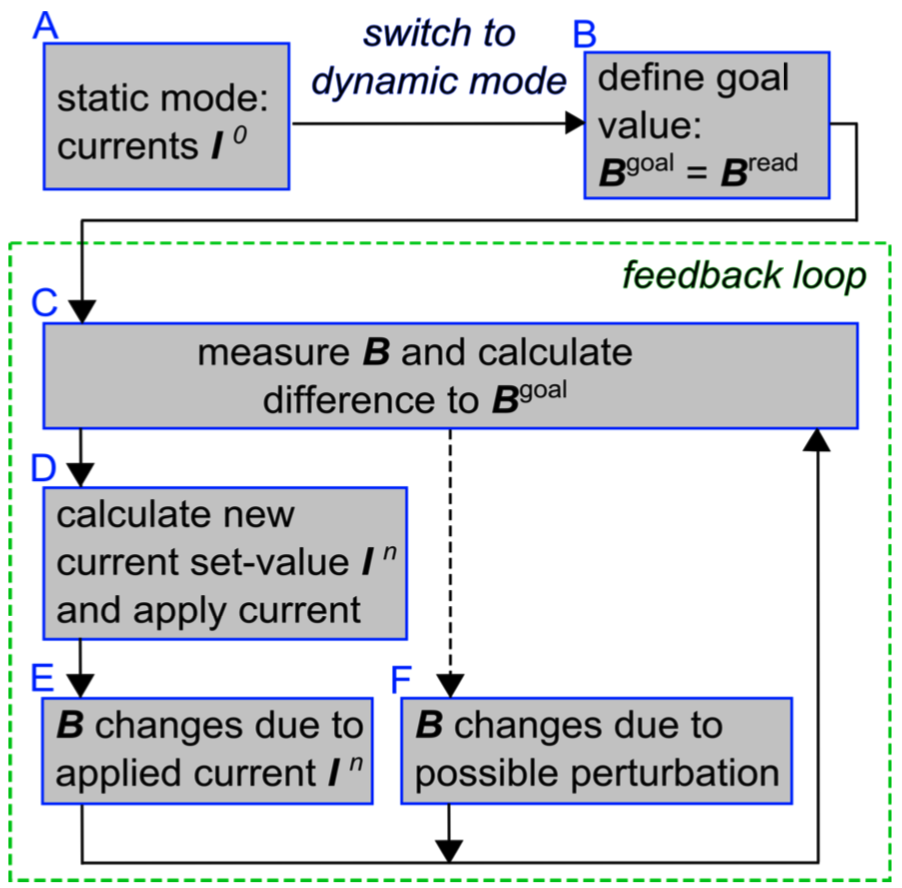
\includegraphics[width=\textwidth]{img/sfc_algorithm}
	\caption{Schematic structure of the SFC lifecycle taken from \cite{Franke2013}.}
	\label{fig:sfc_algorithm}
\end{figure}

\textit{Requirements}: as described in great details in \cite{Franke2013} the SFC system can run in either \texttt{STATIC} or \texttt{DYNAMIC} mode. While in \texttt{STATIC} the system is time-independent and fully characterised with $I^0$ which is a vector with every individual component defining a ratio of the immediate set current in the corresponding coil to the current at the nominal generated magnetic field. When switched to the \texttt{DYNAMIC} mode the new $I^n$ is recalculated on every iteration based on the difference between the expected and the measured fields. An overview of the SFC behaviour in the different modes can be found on the Figure \ref{fig:sfc_algorithm}.

We introduce the following 2 commands to control the experimental setup:
\begin{itemize}
	\item \texttt{MODE <STATIC|DYNAMIC>} that switches between the execution modes.
	\item{
		\texttt{COIL index, current} to modify the components of the $I^0$.
		\begin{itemize}
			\item \texttt{index}, required integer --- an index of the corresponding coil. The coil index itself is derived from the coil's position in the config file. Indices start with 1. Any index that is outside the $I^0$ boundaries is ignored and an error message is printed.
			\item \texttt{current}, required float --- a ratio of the current to be set to the maximal current. However at the moment there are no checks and one can set this value to be greater than 1 if desired.
		\end{itemize}
	}
\end{itemize}

\textit{Implementation details}: existing SFC software communicates with the main \texttt{babySFC.jl} module via a ZeroMQ connection. This endpoint was kept for the sake of the compatibility. However it is important to notice that these ZeroMQ messages simply contain the \textbf{name of the variable} and its new value to be set. Thus one needs to make sure that until the legacy scripts are properly modified to work with the SCPI commands it is necessary to keep the variable name that defines $I^0$ to be \texttt{staticI}.

\subsection{Data interface}
\label{subsec:sfc_data}

\textit{Motivation}: in the n2EDM DAQ system the COM handler is responsible for writing the data to the disk for the further analysis thus it is the job of the SFC to bundle it into a binary message and send the package over TCP.

\textit{Requirements}: we are interested in recording the input and output data of the SFC. The core part of controlling the magnetic field is a set of $N_{coils}$ magnetic coils \cite{Rawlik2018}. Each coil is driven by 3 amplifiers, however this ratio may vary in the future. Every amplifier is connected to a dedicated channel on the Beckhoff EL4134 \cite{BeckhoffDAC2019} analog output terminal, referred later to as the \textbf{DAC module}. There are $N_{modules}^{DAC} = 3$ DAC modules with $N_{channels}^{DAC} = 4$ channels each. The readout of the magnetic field is performed through a set of the $N_{fluxgates}$ triple-axis fluxgates. In total each of the $3 * N_{fluxgates}$ sensors is connected to a separate channel on the Beckhoff EL3602 \cite{BeckhoffADC2019} analog input terminals or the \textbf{ADC modules}. The SFC system operates $N_{modules}^{ADC} = 17$ ADC modules each possessing $N_{channels}^{ADC} = 2$ channels. 

\textit{Implementation details}: let us provide an in-depth analysis of the shape of the data message presented in the Table \ref{tbl:sfc_data_message}.

\renewcommand{\arraystretch}{1.4}
\begin{table}[h]
\centering
\begin{tabular}{|r|l|l|l|}
	\hline
	Amount of fields & Units & Type & Name \\
	\hline \hline
	1 & ns & \texttt{uint64} & \texttt{timestamp} \\
	\hline
	$N_{modules}^{DAC} \times N_{channels}^{DAC}$ & V & \texttt{double} & \texttt{voltage @ dac\_channel\_*} \\
	\hline
	$N_{modules}^{DAC} \times N_{channels}^{DAC}$ & A & \texttt{double} & \texttt{current @ dac\_channel\_*} \\
	\hline
	$N_{modules}^{ADC} \times N_{channels}^{ADC}$ & V & \texttt{double} & \texttt{voltage @ adc\_channel\_*} \\
	\hline
	$N_{coils}$ & \% & \texttt{double} & \texttt{current @ coil\_*} \\
	\hline
\end{tabular}
\caption{Structure of the SFC data message.}
\label{tbl:sfc_data_message}
\end{table}
\renewcommand{\arraystretch}{1}

\begin{itemize}
	\item \texttt{timestamp} --- a UNIX timestamp of the moment when the chunk of data for this message was collected.
	\item \texttt{voltage @ dac\_channel\_*} --- an output voltage in the DAC channel, always 0 if this channel does not have a coil connected.
	\item \texttt{current @ dac\_channel\_*} --- an expected output current of the amplifier connected to the corresponding DAC channel. Always 0 if no connected coil is present.
	\item \texttt{voltage @ adc\_channel\_*} --- a voltage measured in the ADC channel. Either the value read from one of the fluxgate's sensors or noise.
	\item \texttt{current @ coil\_*} --- a ratio of the immediate current in the coil to the current at a generated nominal field.
\end{itemize}

\subsection{Generation of the configs}
\label{subsec:sfc_configs}


\textit{Motivation}: similar to the Feature \ref{subsec:rm-proxy_configs} we have a need to synchronise the configuration between the COM handler and the SFC system. Additionally the data message described in the Feature \ref{subsec:sfc_data} consists of $1 + 2 \times N_{modules}^{DAC} \times N_{channels}^{DAC} + N_{modules}^{ADC} \times N_{channels}^{ADC} + N_{coils} = 62$ fields which makes it unnecessary complicated to be maintained by hand.

\textit{Requirements}: the only scalable and user-friendly way of addressing the problems mentioned above is to resort to programmatic generation of the configuration files. Following the specification \cite{Bison2018} the root config and the configuration file of the COM handler can be consumed by any \texttt{libconfig}-compatible parser. For the SFC itself YAML format was selected due to a better support provided by the Julia programming language.

\textit{Implementation details}: aiming for brevity but without loss of generality we will describe the fields of the reduced (only 1 coil and only 1 fluxgate) root config located in the top level folder of the SFC git repository under the name of \texttt{root\_config.cfg} and presented on the Listing \ref{listing:sfc_root}.

\begin{lstlisting}[
	language=JavaScript,
	caption={Root config of the SFC project.},
	label={listing:sfc_root}
]
moduleName = "SFC";
sfcIpAddress = "127.0.0.1";
sfcScpiPort = 5125;
sfcDataPort = 5126;

inputDelayCycles = 2;
cycleFrequencyHertz = 200;

dacModulesRange = "1:3";
dacChannelsPerModule = 4;

adcModulesRange = "4:20";
adcChannelsPerModule = 2;
adcInputVoltageRange_in_V = 5;

coils = (
    {
        name: "X",
        amplifiers: (
            {
                dacChannelNumber: 1,
                dacOutputVoltageAtNominalField_in_V: 5,
                amplifierGain_in_AmperPer10Volt: 10
            },
            {
                dacChannelNumber: 5,
                dacOutputVoltageAtNominalField_in_V: 1,
                amplifierGain_in_AmperPer10Volt: 2
            },
            {
                dacChannelNumber: 9,
                dacOutputVoltageAtNominalField_in_V: 0.1,
                amplifierGain_in_AmperPer10Volt: 0.4
            }
        )
    }
);

fluxgates = (
    {
        name: "1",
        location: "top",
        channels: {
            x: 1,
            y: 2,
            z: 3
        }
    }
)
\end{lstlisting}

\begin{itemize}
	\item \texttt{moduleName}, required string --- an identifier for the COM handler within the n2EDM DAQ system. Is provided to the distributor.
	\item \texttt{sfcIpAddress}, required string --- an IP address of the SFC system relative to the COM handler.
	\item \texttt{sfcScpiPort} and \texttt{sfcDataPort}, required integers --- the ports for the SCPI and data connections, respectively. TCP server of the SFC awaits for the TCP client of the COM handler on them.
	\item \texttt{inputDelayCycles}, required integer --- an empirical value of the delay between setting the voltages in the DAC and reading the field change in the ADC.
	\item \texttt{cycleFrequencyHertz}, required integer --- a frequency of the SFC feedback and data collection loop.
	\item \texttt{dacModulesRange}, required string --- a Julia-inspired \cite{Juliacontributors} range describing the position of the DAC modules in the device chain. Enumeration starts with 1, last value is included. Only a \texttt{start:end}, where $\texttt{start} < \texttt{end}$, format is supported. It is expected that both the DAC and the ADC modules are installed in homogeneous blocks with the ADC partition immediately following the DAC region. This allows us to address the DAC and ADC channels without the need to specify the module position. For example, a channel 1 in the DAC module 2 can be targeted with $\texttt{dacChannelNumber} = 5$ (see below in the \texttt{coils} section). Same approach is used for the ADC channels in the \texttt{fluxgates} section of the present configuration file. Just like the indexing of the modules themselves, the independent indexing of the DAC and ADC channels starts with 1.
	\item \texttt{dacChannelsPerModule}, required integer --- self-explanatory, is 4 for the Beckhoff EL4134 \cite{BeckhoffDAC2019}.
	\item \texttt{adcModulesRange}, required string --- follows the specification described for the \texttt{dacModulesRange} but characterises the ADC modules. 
	\item \texttt{adcChannelsPerModule}, required integer --- self-explanatory, is 2 for the Beckhoff EL3602 \cite{BeckhoffADC2019}.
	\item \texttt{adcInputVoltageRange\_in\_V}, required integer --- defines the input voltage range of all ADC modules.
	\item{
		\texttt{coils}, required array --- describes the controlled magnetic coil. Contains the objects with the following set of fields:
		\begin{itemize}
			\item \texttt{name}, required string --- a human-readable identifier of the coil, it is included into the generated COM handler's config for the data analysis.
			\item{
				\texttt{amplifiers}, required array --- describes the amplifiers driving this coil. The children have these fields:
				\begin{itemize}
					\item \texttt{dacChannelNumber}, required integer --- a number of the DAC channel managing this amplifier. Must be consistent with the specification presented at the \texttt{dacModulesRange} description.
					\item \texttt{dacOutputVoltageAtNominalField\_in\_V}, required integer -- an output voltage of this DAC channel when the corresponding coil is set to generate the nominal field. In the \texttt{STATIC} mode this SCPI command from the Feature \ref{subsec:sfc_scpi} would set this voltage value: "\texttt{COIL coil\_index, 1}".
					\item \texttt{amplifierGain\_in\_AmperPer10Volt}, required integer --- is used to characterise the connected amplifier.
				\end{itemize}
			}
		\end{itemize}
	}
	\item{
		\texttt{fluxgates}, required array --- depicts the fluxgates used to read out the magnetic field. Encloses the objects with the following properties:
		\begin{itemize}
			\item \texttt{name}, required string --- a label used to distinguish different fluxgates. Is included into the COM handler's config for the further data analysis.
			\item \texttt{location}, required string --- relates to the physical location of the fluxgate. Is also included in the COM handler's configuration file.
			\item \texttt{channels}, required object --- an object with the keys \texttt{x}, \texttt{y}, and \texttt{z} in a flexible order. Every value of the subfield corresponds to the ADC channel connected to measure the related component of the magnetic field. The channel numbers conform to the specification introduced in the \texttt{dacModulesRange} decription.
		\end{itemize}
	}
\end{itemize}

Executing the command below from the SFC repository root
\begin{verbatim}
python3 ./generate_configs.py
\end{verbatim}
would read \texttt{./root\_config.cfg} and create or overwrite 2 configs:
\begin{itemize}
	\item \texttt{generated/conf\_sfc.yaml} is for the SFC system.
	\item \texttt{generated/conf\_n2comhandler.cfg} is for the COM handler.
\end{itemize}








